\section{Instruções}
O código é acompanhado de um arquivo Makefile para sua execução. Ele imprime duas árvore B, uma com chaves "int" e grau mínimo 3 e outra com chaves "char" e grau mínimo 2. Ela está configurada para rodar com "char".
\par Para trocar o tipo e o grau mínimo da árvore, é necessário modificar os arquivos arvoreb.h, mainArvoreb.c, printArvoreb.c e removeArvoreb.c. No arquivo arvoreb.h, altere onde estão circulados em vermelho na imagem para o tipo e grau mínimo desejado.

\begin{figure}[!h]
\centering
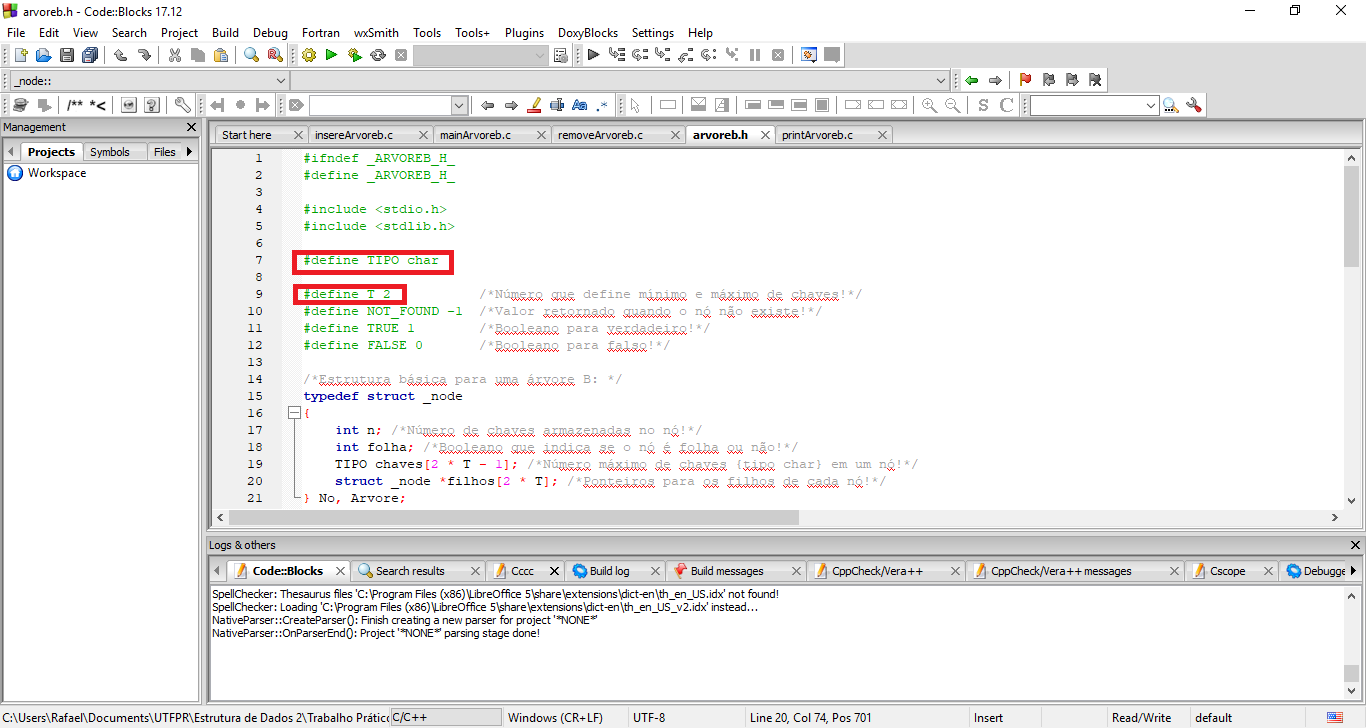
\includegraphics[width=6in]{relatorio/imagens/imgMudarTipoH.png}
\end{figure}

\newpage

\par No arquivo mainArvoreb.c, dentro da main, remova os comentários da função equivalente ao tipo que você quer (Numérico = "int", Alfabeto = "char"), como indica a figura abaixo no retângulo vermelho:

\begin{figure}[!h]
\centering
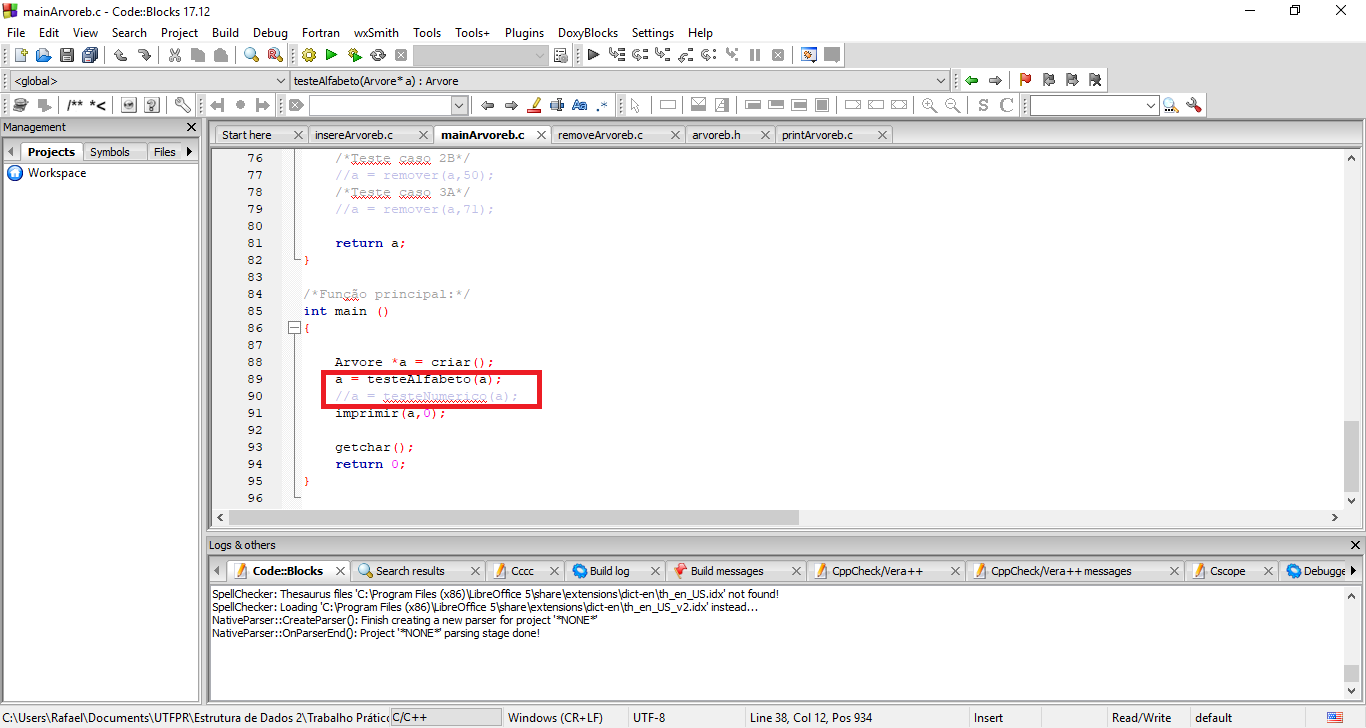
\includegraphics[width=6in]{relatorio/imagens/imgMudarTipoMain.png}
\end{figure}

\par Em printArvoreb.c, basta alterar alterar o tipo de sáida do printf circulado em vermelho na imagem abaixo para corresponder ao tipo da sua árvore:

\begin{figure}[!h]
\centering
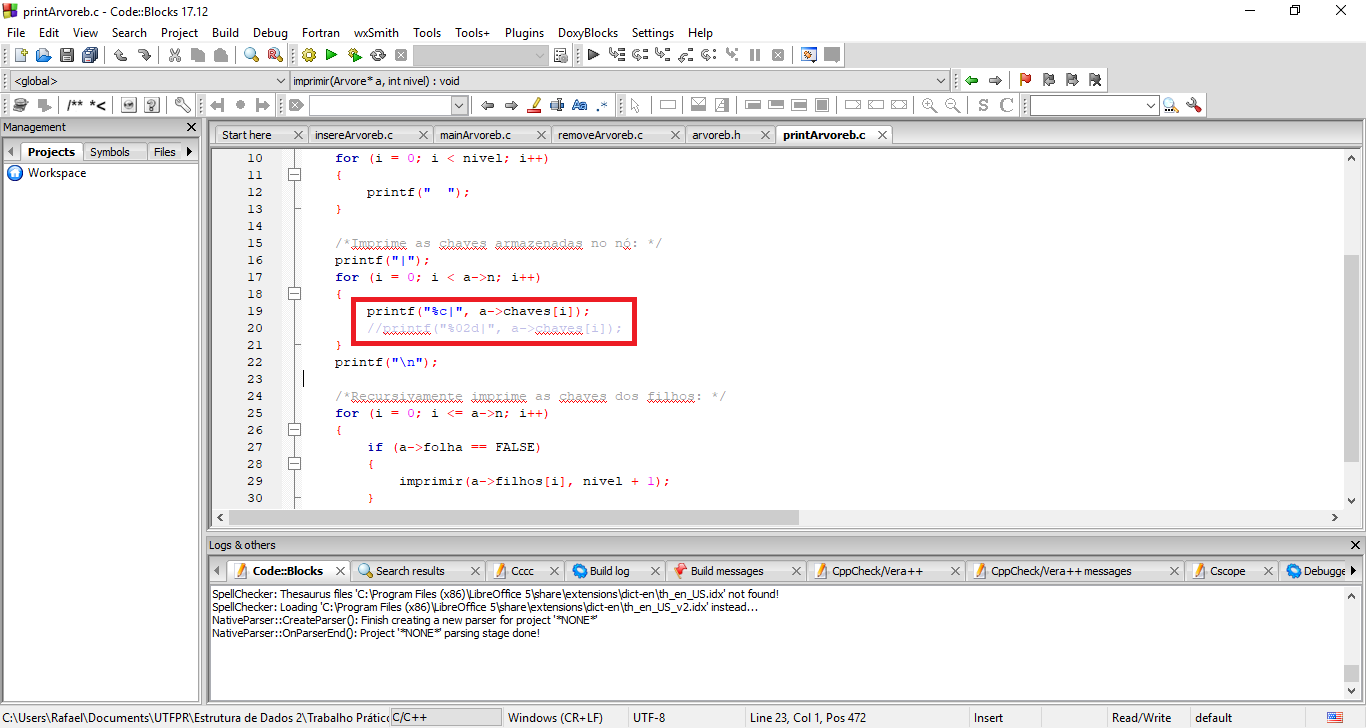
\includegraphics[width=6in]{relatorio/imagens/imgMudarTipoPrint.png}
\end{figure}
\newpage
\par Enfim, para removeArvoreb.c, basta fazer a mesma coisa que em printArvoreb.c:

\begin{figure}[!h]
\centering
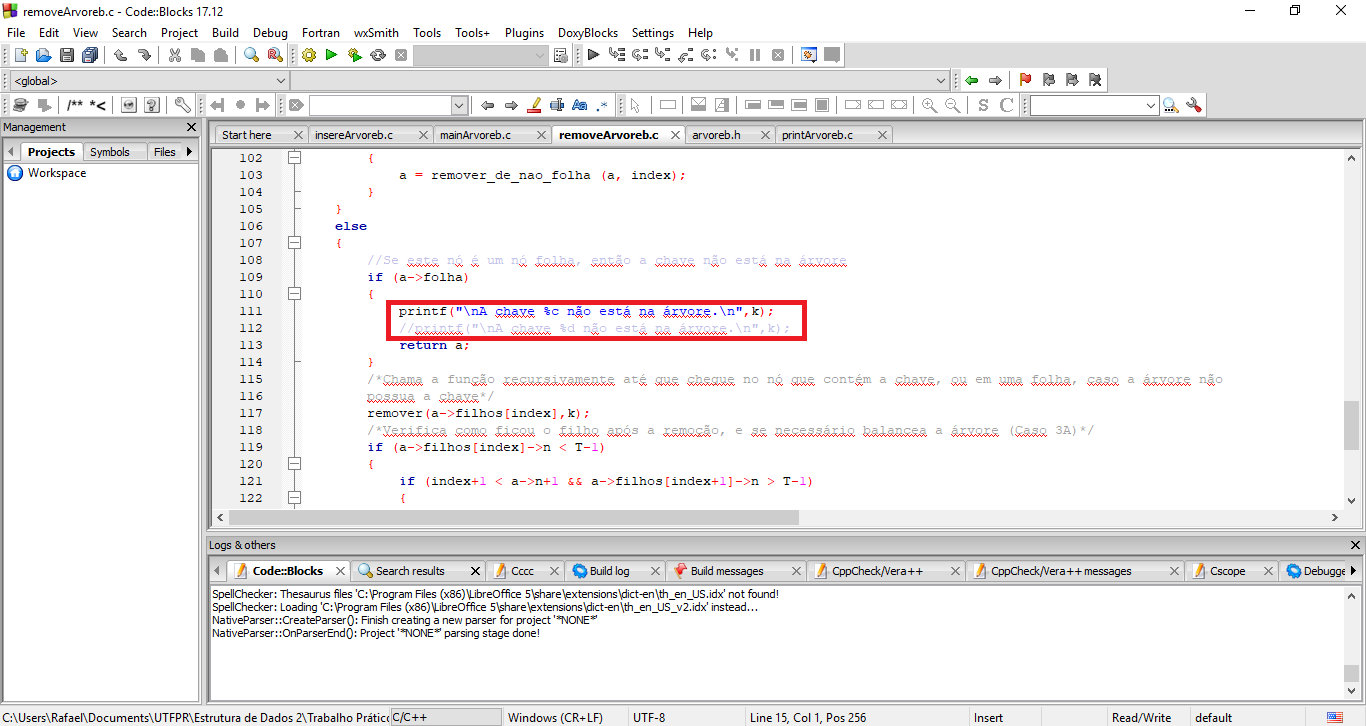
\includegraphics[width=6in]{relatorio/imagens/imgMudarTipoRemove.png}
\end{figure}
\par Nosso código também vem com alguns testes de remoção. Eles se encontram dentro das funções testeAlfabeto e testeNumerico, ambas com seus respectivos testes. Para realizar uma remoção, basta tirar do comentário qualquer uma das chamadas de remoção, mas como nosso programa só implementou 4 formas de remoção, pode causar problemas rodar mais do que uma na mesma execução. Recomendamos que se teste uma por vez.

\begin{figure}[!h]
\centering
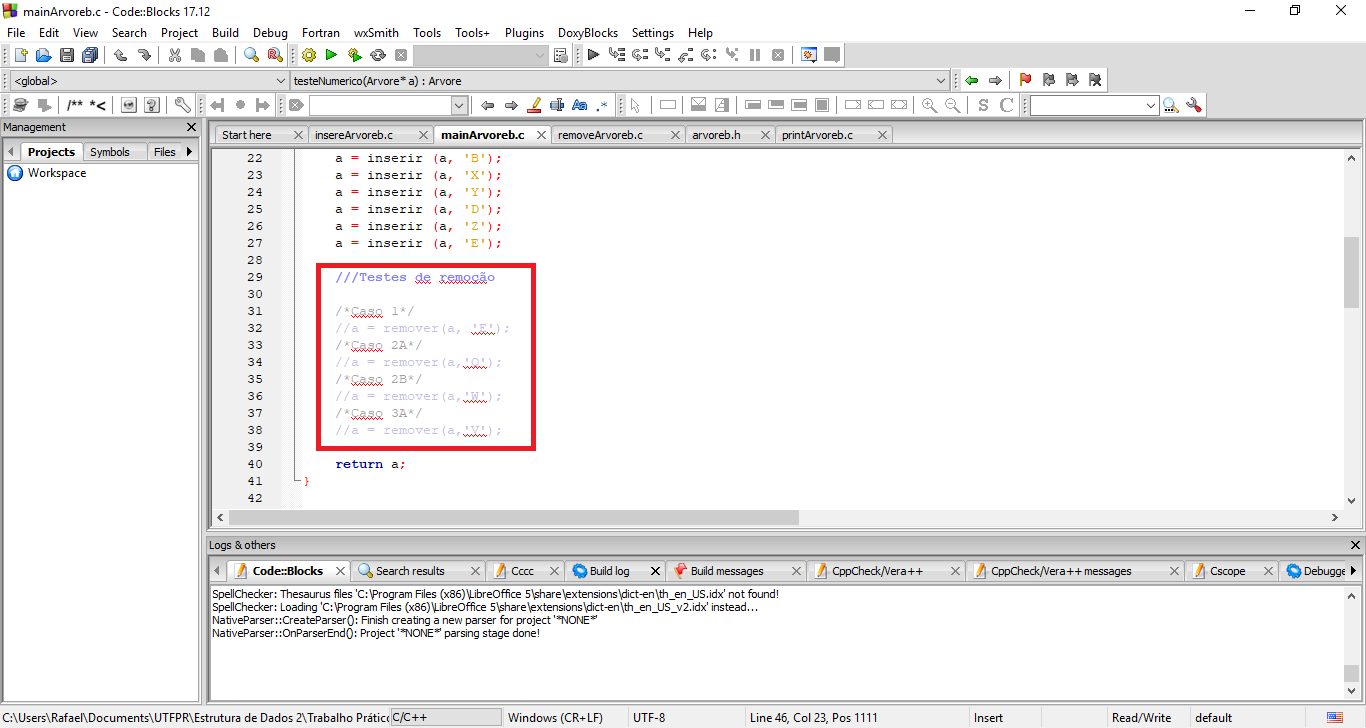
\includegraphics[width=6in]{relatorio/imagens/imgTestesRemocaoChar.png}
\end{figure}

\begin{figure}[!h]
\centering
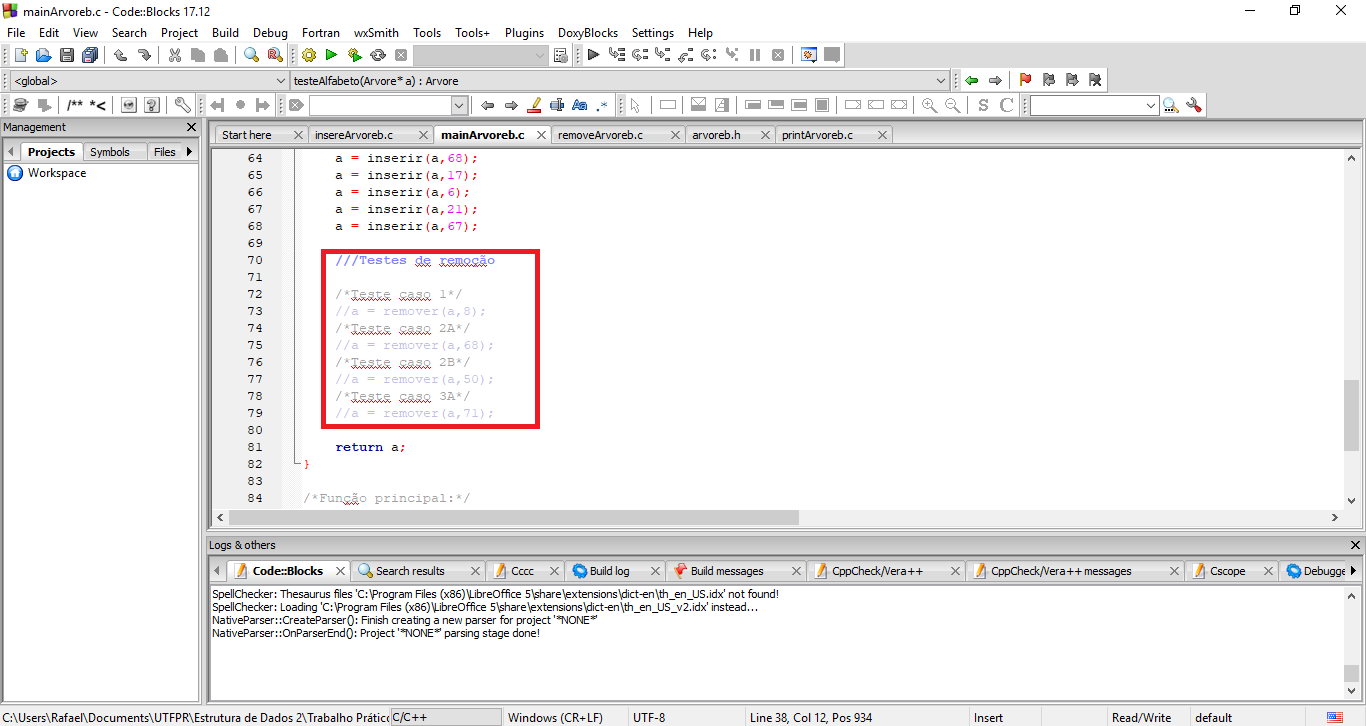
\includegraphics[width=6in]{relatorio/imagens/imgTestesRemocaoInt.png}
\end{figure}